\section{Solution Class Reference}
\label{classSolution}\index{Solution@{Solution}}
Inheritance diagram for Solution::\begin{figure}[H]
\begin{center}
\leavevmode
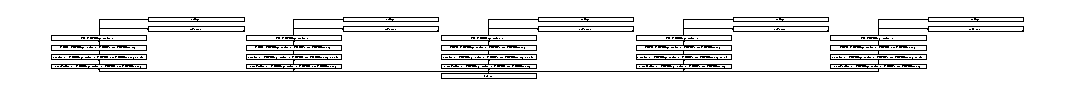
\includegraphics[height=0.823529cm]{classSolution}
\end{center}
\end{figure}
\subsection*{Public Member Functions}
\begin{CompactItemize}
\item 
\bf{Solution} ()\label{classSolution_b55bd4b023d596ce11aaf737b9a6123b}

\item 
\bf{Solution} ()\label{classSolution_b55bd4b023d596ce11aaf737b9a6123b}

\item 
\bf{Solution} ()\label{classSolution_b55bd4b023d596ce11aaf737b9a6123b}

\item 
\bf{Solution} ()\label{classSolution_b55bd4b023d596ce11aaf737b9a6123b}

\item 
\bf{Solution} ()\label{classSolution_b55bd4b023d596ce11aaf737b9a6123b}

\end{CompactItemize}


\subsection{Detailed Description}




Definition at line 66 of file t-moeo\-Easy\-EA.cpp.

The documentation for this class was generated from the following files:\begin{CompactItemize}
\item 
t-moeo\-Easy\-EA.cpp\item 
t-moeo\-IBEA.cpp\item 
t-moeo\-Max3Obj.cpp\item 
t-moeo\-NSGA.cpp\item 
t-moeo\-NSGAII.cpp\end{CompactItemize}
